\documentclass[12pt,a4j]{jsarticle}

\usepackage[dvipdfmx]{graphicx}
\usepackage[top=15truemm,bottom=15truemm,left=15truemm,right=15truemm]{geometry}
\usepackage{amsmath}
\usepackage{txfonts}
\usepackage{array}
\renewcommand{\ }{\hspace{1zw}}

\title{頭部回転による音像定位精度の変化}
\author{先端音情報システム研究室 修士2年 前田啓}
\date{2019/6/14}

\begin{document}
\maketitle
\section{研究背景}
音を聞いたとき,それがどこから聞こえてきたか(音源がどこにあるか)を知覚することを音像定位と呼ぶ.
後方の危険察知や集団でのコミュニケーションを含め,音を聞くあらゆる場面において音像定位能力の果たす役割は非常に大きい.

水平方向の定位には両耳に到達する音の時間差と強度差が重要である.
それぞれを両耳間時間差(Interaural Time Difference; ITD)・両耳間強度差(Interaural Intensity Difference; IID)と呼ぶ.
一方仰角方向の定位には頭部伝達関数(Head-Related Transfer Fuction; HRTF)が重要である.
頭部伝達関数とは音源から外耳道入り口への音響的な伝達関数を表し,耳介や頭部・肩などの身体形状に起因するため,個人差が大きい.

音像定位において音が重要であることは明らかだが,これまでに,音だけではなく他感覚情報も統合して方向定位が行われることが知られている.
例えば,音声刺激が見えている話者の方向から聞こえる腹話術効果(ventriloquism effect)は,視覚情報が音像定位に影響する例と言える.
音情報と前庭感覚情報を動的に変えうる運動の代表例として,頭部運動が挙げられる.
頭部運動は,うなずき(nodding),かしげ(pivoting),回転(rotating)の三方向の運動に分けられるが,中でも回転は頭部に対する音源の相対的な位置を変化させると同時に,回転感覚を生起させる.
そのため,頭部運動が音像定位に影響することが予想される.

頭部回転と音像定位の関係を調べた実験は多数あるが,その方法によって,「頭部回転によって音像定位能力が向上する」という結果と,「音像定位能力が悪化する」という結果の真逆のような二種類に分けられる.
例えば,改善例として,ヘッドホン提示において,まるで実空間聴取のように,頭部回転にともない対応する角度のHRTFを畳み込んだところ,前後誤判断が減少した\cite{Kawaura}.
また,回転方向のトレースによって水平面定位精度が改善すること\cite{Iwaya}や,自由に頭部運動できるときには頭外定位の比率が上昇すること\cite{Brimijoin}が報告されている.
以上の実験では,いずれも頭部運動がひと段落してから回答させている.
一方で,頭部回転によって音像定位精度が悪化する例としては,頭部回転の後半に音提示すると定位誤差が増加すること\cite{Cooper}や,仮想音源の移動検知限が頭部回転中に増加すること\cite{Honda},受動全身回転中は速度にかかわらず主観的正面の弁別限が増加すること\cite{Masumi}\cite{Tsuno}が知られている.
定位精度が悪化した実験に共通するのは,いずれも頭部回転の最中に音像定位させたことである.

以上に述べたような改善・悪化の二種類の現象が起きる理由は未だに明らかになっていない.
頭を動かしながら音を聞くというありふれた場面での聴覚の性質を解明することは,より高い臨場感を提示する音再生技術の発展に不可欠だと筆者は考える.

\section{研究目的}
研究目的は,頭部回転の最中に音像定位精度が悪化する原因を明らかにすることである.
受動全身回転中は主観的正面の弁別限が増加することが知られている.
%これまでに,回転速度・刺激音の長さ・暗闇時間の長さ・音提示前の回転などの影響が調査されたが,いずれも定位精度悪化の原因解明には至っていない.
過去に定位精度の悪化が確認された実験ではいずれも頭部回転の最中に定位・回答を課されていたことと,最近の実験で回転速度や試験音の長さ・音提示前の回転は定位精度に影響しないことが示されたことから,精度悪化の原因の候補として回転感覚と相対的な音方向の変化(ITD・IIDの時間変化)が挙げられる.
そこで本研究では,頭部回転中の音像定位精度変化原因として,相対的な音方向変化と回転感覚の妥当性を調べる.

\section{ベクション生起中の音像定位実験}
通常の頭部回転では,ITD・IIDが経時的に変化すると同時に,前庭感覚への入力により回転感覚が生じる.
それぞれが音像定位にもたらす影響を調べるには,片方のみを知覚している最中の音像定位実験を行う必要がある.
そこで,ヘッドマウントディスプレイを用いたベクション生起中の音像定位実験を行うことで,回転を知覚しながら相対的な音方向は変化しない状況での定位精度を調べた.

本実験で用いた機器は,ラウドスピーカ,Oculusヘッドマウントディスプレイ,Oculusコントローラー,フットペダルであった.
ラウドスピーカは被験者の物理的正面に対して左右9$^\circ$の範囲に,2$^\circ$間隔で10個配置した.
実験条件は,静止条件と,ベクション条件の二種類とした.
被験者は3名で,このうち2名(被験者1, 2)は静止条件から,残りの1名はベクション条件から先に実験を行った.
本実験系を以下に示す.
\begin{figure}[htbp]
    \centering
    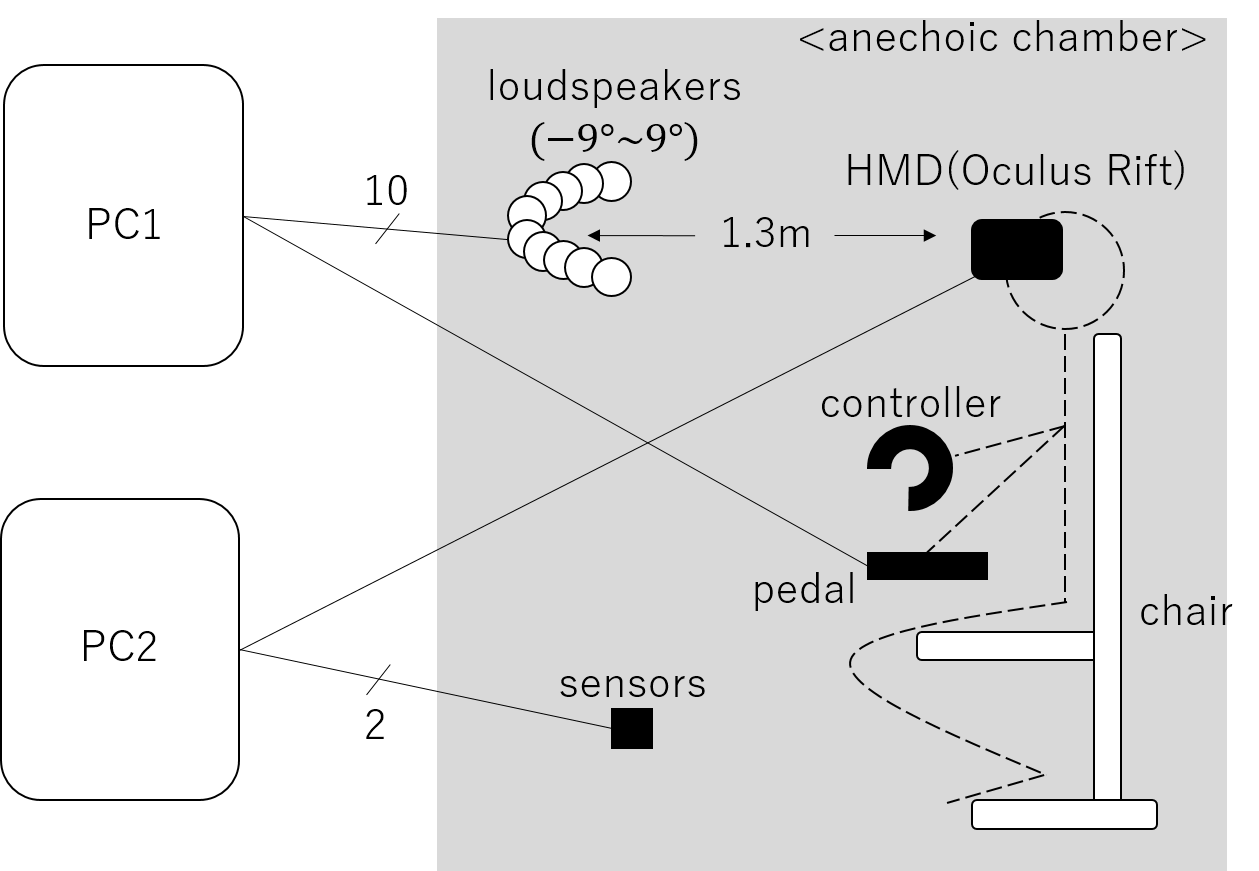
\includegraphics[width=0.8\columnwidth]{./figure/system.png}
    \caption{実験系}
    \label{system}
\end{figure}

\raggedright
\subsection{静止条件}
\ この条件では,ヘッドマウントディスプレイを用いて,固視点を提示したのち,同一球面上で静止する複数の球の映像を提示した.
背景は暗闇で,固視点として赤い十字を被験者の物理的正面(ラウドスピーカアレイの中心と一致)に配置した.
固視点を30 s間見せたのち,被験者を中心とした半径5 mの球上に直径20 cmの球が10000個ランダムに配置された映像を提示した.
このとき,球はすべて静止させた.
被験者には頭と目を動かさず固視点の方向を見続けるよう指示した.
球の映像に切り替わったら,ひとつのラウドスピーカから30 msのピンクノイズ(連続提示時65 dBとなるよう校正)を提示した.
提示スピーカは,ランダム化最尤適応法によって決定した.
試験音が主観的正面に対し左右どちらから聞こえたかを,二肢強制選択で回答させた.
試行回数は計100回で,2セッション各50回に分けて実施した.
被験者は筆者を含む三名であった.

\subsection{ベクション条件}
\ この条件では,固視点を提示したのち,同一球面上の複数の球が左右どちらかすべて同じ方向に定速移動する映像を提示した.
球の映像に切り替わったのち,被験者がまるでその場で回転しているように感じたら手元のボタンを押すように指示した.
ボタン応答を感知したら,ひとつのラウドスピーカから静止条件で用いたものと同じ試験音を提示し,左右どちらから聞こえたかを二肢強制選択で回答させた.
また,球の映像に切り替わった時刻とボタン応答の時刻を記録し差を求めることで,ベクション生起にかかった時間を測定した.
試行回数は計200回(球移動方向各100回)で,4セッション各50回に分けて実施した.
被験者は静止条件を受けた者と同じ三名であった.

\subsection{結果}
\ 各提示位置において右から聞こえたと回答した比率に累積正規分布曲線を当てはめることで,心理測定関数を推定した.
平均値をPSE,標準偏差の0.6745倍の値をjndと定めた.
本実験においては,PSEは主観的正面,jndは定位精度の悪さを表す指標とみなすことができる.
静止条件における三名分の心理測定関数を示す.
\begin{figure}[htbp]
    \centering
    \begin{tabular}{ccc}
        \begin{minipage}{0.33\columnwidth}
            \centering
            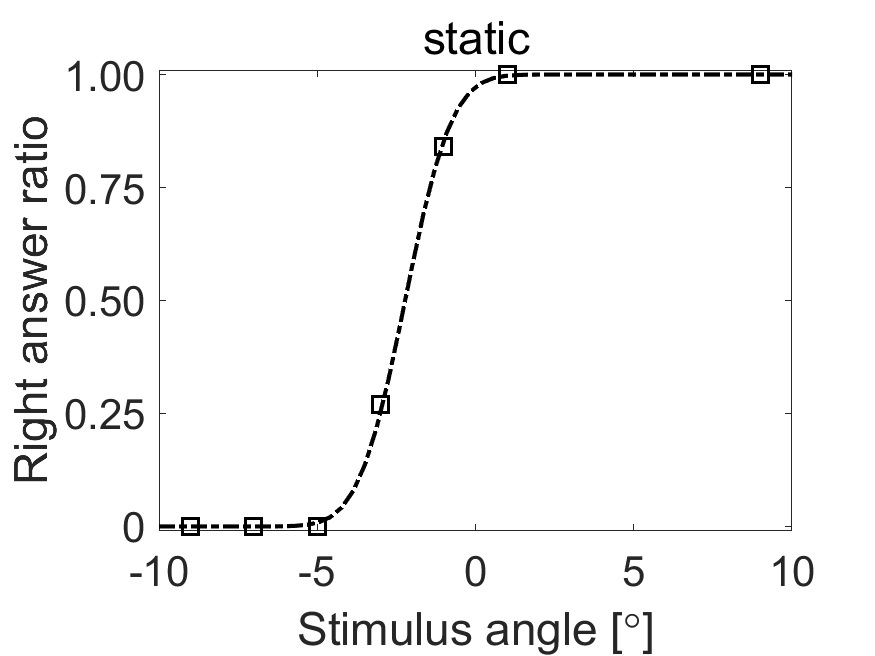
\includegraphics[width=\columnwidth]{./figure/NoMove_maeda.png}
            Subject 1
        \end{minipage}
        \begin{minipage}{0.33\columnwidth}
            \centering
            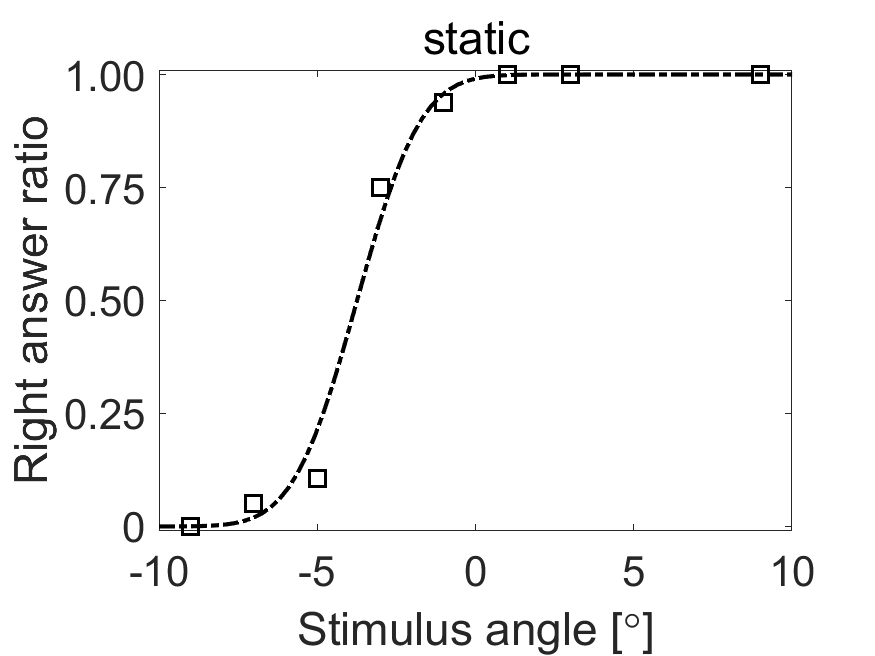
\includegraphics[width=\columnwidth]{./figure/NoMove_niitsuma.png}
            Subject 2
        \end{minipage}
        \begin{minipage}{0.33\columnwidth}
            \centering
            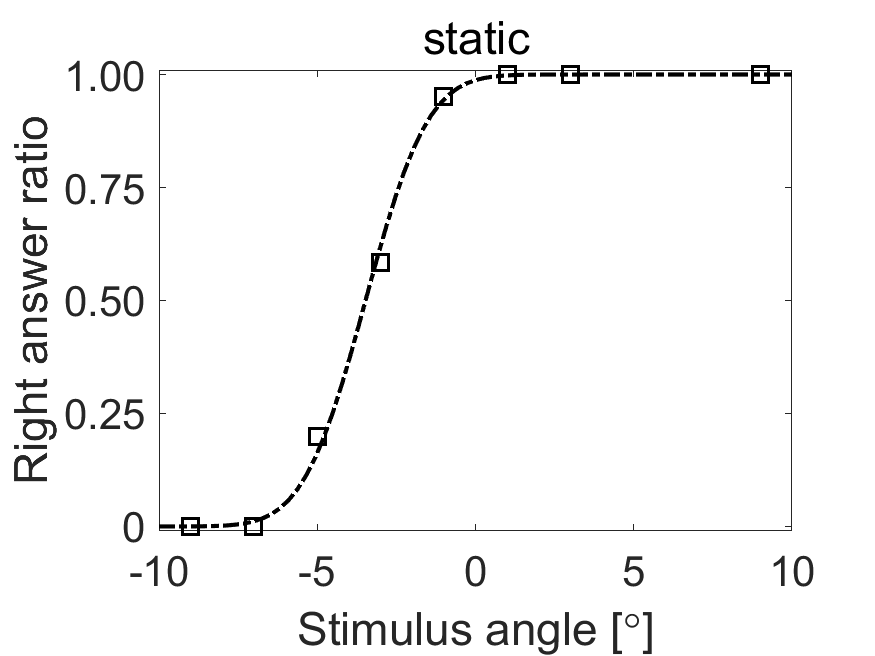
\includegraphics[width=\columnwidth]{./figure/NoMove_oikawa.png}
            Subject 3
        \end{minipage}
    \end{tabular}
    \caption{心理測定関数(静止条件)}
    \label{pf_s}
\end{figure}

\raggedright
次に,ベクション条件の心理測定関数を示す.
\begin{figure}[htbp]
    \centering
    \begin{tabular}{ccc}
        \begin{minipage}{0.33\columnwidth}
            \centering
            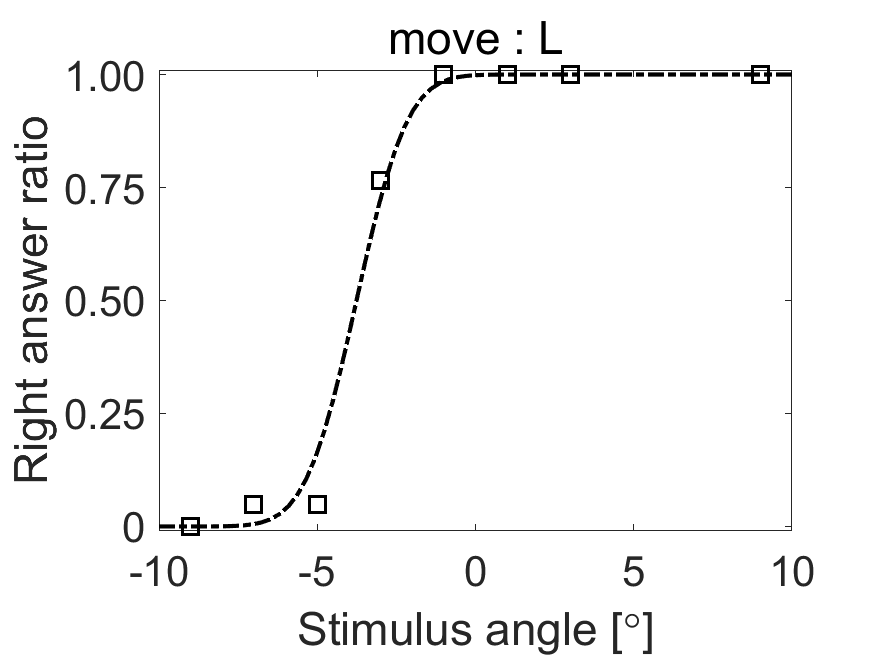
\includegraphics[width=\columnwidth]{./figure/L_maeda.png}
            Subject 1 (L)
        \end{minipage}
        \begin{minipage}{0.33\columnwidth}
            \centering
            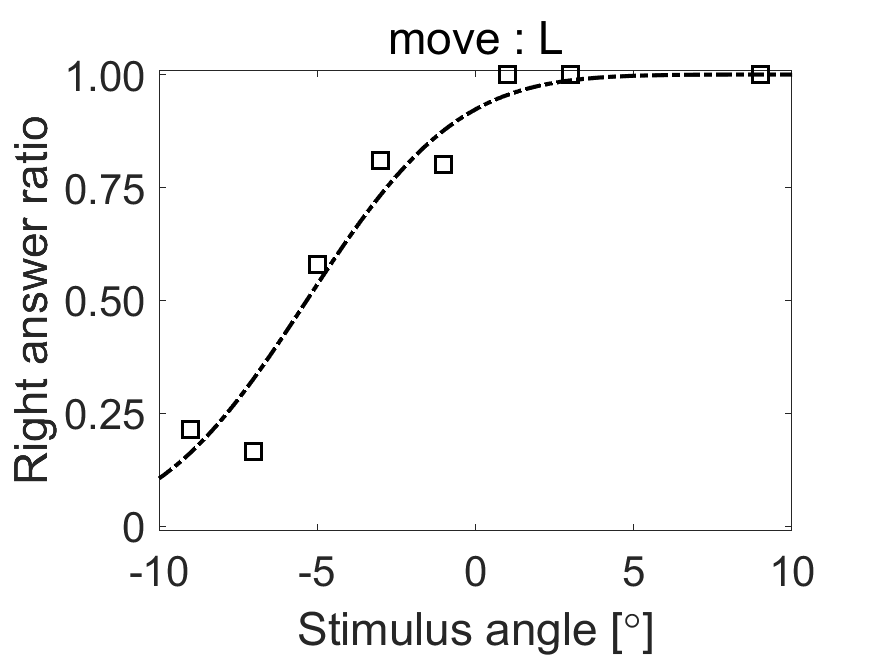
\includegraphics[width=\columnwidth]{./figure/L_niitsuma.png}
            Subject 2 (L)
        \end{minipage}
        \begin{minipage}{0.33\columnwidth}
            \centering
            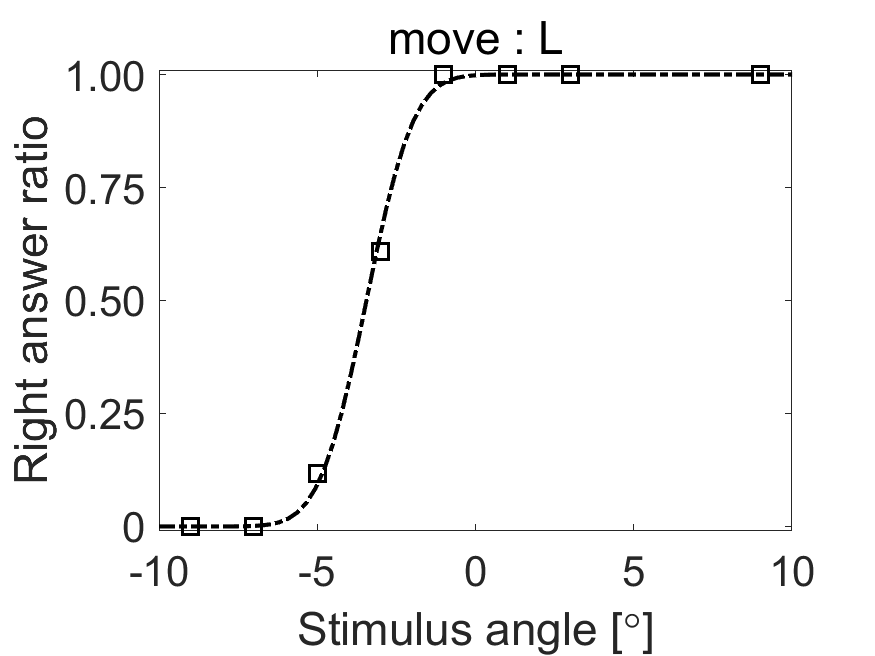
\includegraphics[width=\columnwidth]{./figure/L_oikawa.png}
            Subject 3 (L)
        \end{minipage}\\
        \vspace{0.5cm}
        \begin{minipage}{0.33\columnwidth}
            \centering
            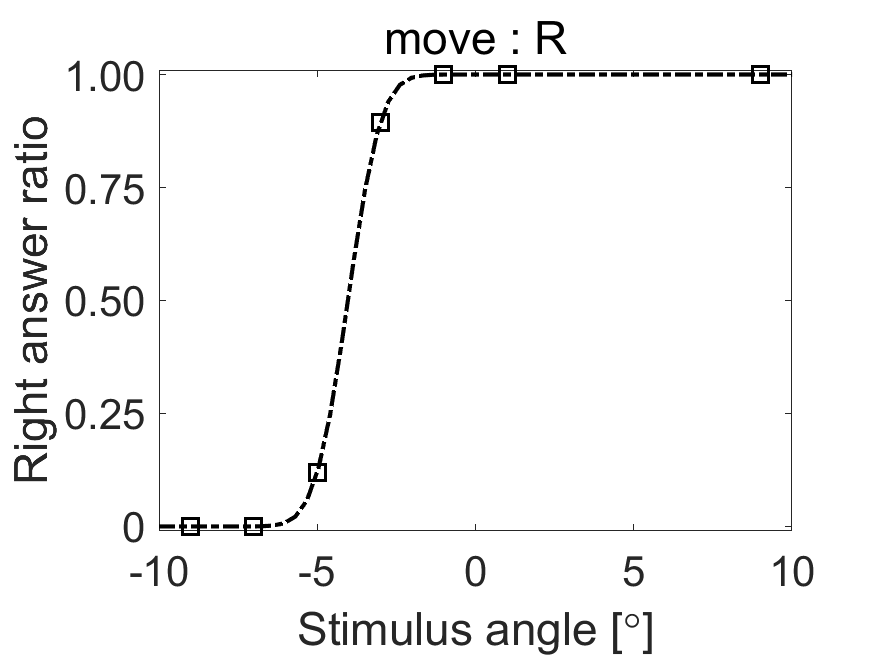
\includegraphics[width=\columnwidth]{./figure/R_maeda.png}
            Subject 1 (R)
        \end{minipage}
        \begin{minipage}{0.33\columnwidth}
            \centering
            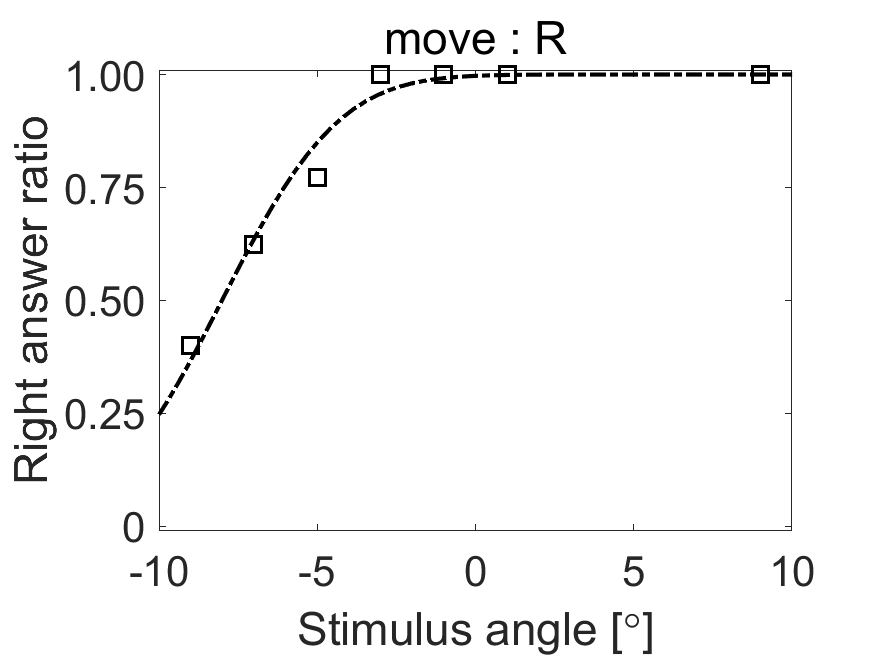
\includegraphics[width=\columnwidth]{./figure/R_niitsuma.png}
            Subject 2 (R)
        \end{minipage}
        \begin{minipage}{0.33\columnwidth}
            \centering
            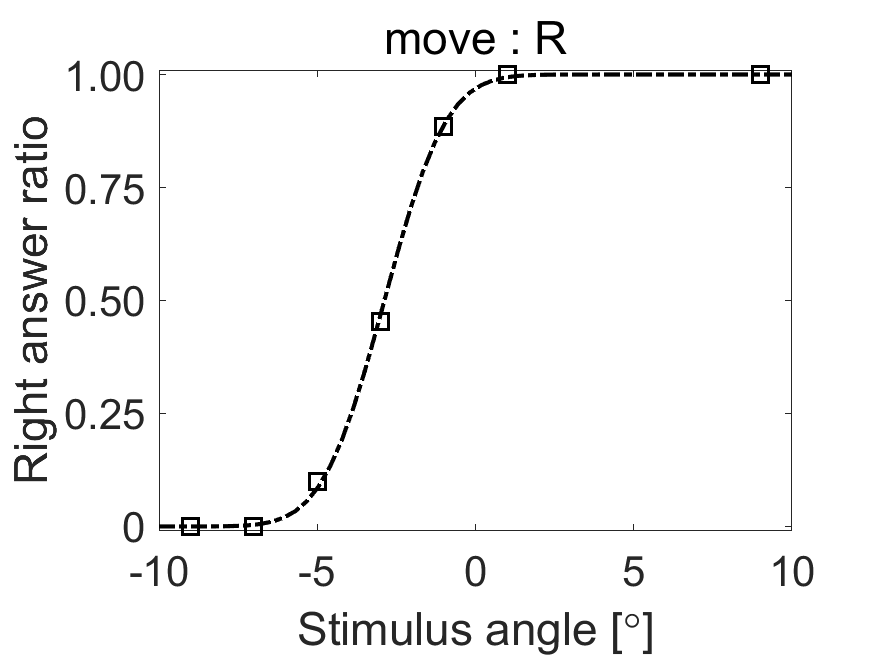
\includegraphics[width=\columnwidth]{./figure/R_oikawa.png}
            Subject 3 (R)
        \end{minipage}
    \end{tabular}
    \caption{心理測定関数(静止条件)}
    \label{pf_v}
\end{figure}

\raggedright
以上の推定で得たPSEとjndを表\ref{table}にまとめる.
% Excel で表を作成しpngを挿入
\begin{table}[htbp]
    \centering
    \caption{推定したPSEとjnd}
        \begin{tabular}{|c|c||r|r|r|}\hline
            \multicolumn{2}{|c||}{} & static & \multicolumn{2}{c|}{vection}\\
            \cline{4-5}
            \multicolumn{2}{|c||}{} &  & \multicolumn{1}{c|}{L} & \multicolumn{1}{c|}{R}\\ \hline \hline
             & subject 1 & -2.22 & -3.76 & -4.03 \\ \cline{2-5}
            PSE [$^\circ$] & subject 2 & -3.74 & -5.33 & -8.01\\ \cline{2-5}
             & subject 3 & -3.47 & -3.45 & -2.88 \\ \hline
             & subject 1 & 0.78 & 0.85 & 0.55 \\ \cline{2-5}
            jnd [$^\circ$] & subject 2 & 1.07 & 2.52 & 1.96 \\ \cline{2-5}
             & subject 3 & 1.04 & 0.79 & 1.04 \\ \hline
        \end{tabular}
    \label{table}
\end{table}

\raggedright
PSEの値がすべて負になっているのは,最初に提示する固視点がアレイ中心からずれていたことが原因として考えられ,修正する必要がある.
次にjndについて,subject 1とsubject 3は静止条件とベクション条件でそれほど変わらなかったのに対し,subject 2はベクション条件で倍近く増加している.
現時点では被験者が非常に少ないため統計検定を行っていないが,今後被験者を増やして静止条件とベクション条件の間に定位精度の差があるかどうかを調査する予定である.

\ 続いて,ベクション生起にかかった時間を図\ref{vt}に示す.
\begin{figure}
    \begin{tabular}{cc}
        \begin{minipage}{0.5 \columnwidth}
            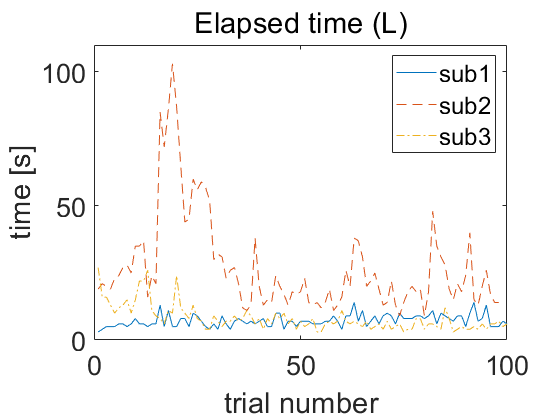
\includegraphics[width=\columnwidth]{./figure/allVT_L.png}
        \end{minipage}
        \begin{minipage}{0.5 \columnwidth}
            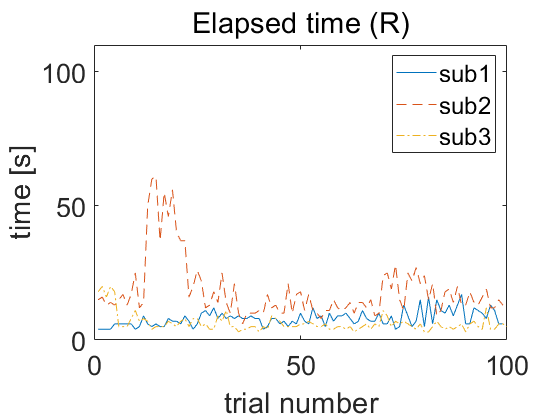
\includegraphics[width=\columnwidth]{./figure/allVT_R.png}
        \end{minipage}
    \end{tabular}
    \caption{ベクション生起にかかった時間}
    \label{vt}
\end{figure}
この図によると,ベクション生起にかかる時間に時間差はあるが,およそ10$\sim$100秒に収まっており,今後も実験時間が長くなりすぎることはないと予想している.

\section{今後の予定}
\ まず,より正確なPSEの推定のために固視点のずれを修正する.
また,ベクション刺激において球がより近くで移動するほうがベクションが生起しやすいかもしれないと考え,球を直径10 cm・周囲5 m配置から,直径5 cm・周囲2 m配置に変更する.
さらに,球が移動する映像を見せたときに生じるベクションが回転運動ではなく真横移動である可能性もあるため,ベクション条件のボタン応答における教示を,「その場で回っているように感じたらボタンを押す」から,「その場で動いているように感じたら」とし,実験後にどのような運動を知覚していたか質問するように手順を変更する.
今後,二十名程度の被験者を募集する予定である.

\begin{thebibliography}{1}
    % \bibitem{ITDs} Brian C. J. Moore, ``Psychology of Hearing (Sixth Edition),'' 248-249, 2013.
    \bibitem{Kawaura} J. Kawaura {\it et al.}, ``Sound localization in headphone reproduction by simulating transfer functions from the sound source to the external ear,'' {\it Acoust. Soc. Jpn.(E)}, 1989.
    \bibitem{Iwaya} Y. Iwaya {\it et al.}, ``Effect of Listener's Head Movement on the Accuracy of Sound Localization in Virtual Environment,'' {\it Acoust. Sci. \& Tech.}, 24, 322-324, 2004.
    \bibitem{Brimijoin} W. O. Brimijoin {\it et al.}, ``The contribution of head movement to the externalization and internalization of sounds,'' {\it PLoS ONE}, 8, 2015.
    \bibitem{Cooper} J. Cooper {\it et al.}, ``Distortions of sound image movement during horizontal head rotation,'' {\it Exp. Brain Res}., 191, 209-219, 2008.
    \bibitem{Honda} A. Honda {\it et al.}, ``Detection of sound image movement during horizontal head rotation,'' {\it i-perception}, 7, 2041669516669614, 2016.
    \bibitem{Masumi} Y. Masumi {\it et al.}, ``Listener's subjective front in horizontal sound localization: Effects of head movements and face directions,'' {\it 2014 RISP International Workshop on Nonlinear Circuits, Communication and Signal Processing}, 2014.
    \bibitem{Tsuno} 角掛沙也香ら,``聴取者受動回転時における音像定位精度の回転速度依存性の検討,'' 音講論,2016.
\end{thebibliography}
\end{document}